%DLC development

\begin{frame}{Features of DLC in APP}
    \begin{minipage}[c]{0.64\textwidth}
        \begin{itemize}
            \item Constantly growing precission and data amounts;
            \item Rare events and low statistics;
            \item Call for multi-messenger astrophysics;
            \item Need for various data in analysis;
            \item Data mining in astroparticle data;
            \item Need for advanced storage architectures and smart data selection queries.

        %     \item Experiments improve and are measuring events with greater precision (large amount of data);
        %     \item But not too many events of our interest;
        %     \item[$\Rightarrow$] combined analysis of data from different experiments becomes topical;
        %     \item Astronomical Virtual Observatories (Auger \& IceCube data).


        %     \item  constantly growing precission and data amounts;
        %     \item rare events and low statistics;
        %     \item call for multi-messenger astrophysics;
        %     \item  need for various data in analysis;
        %     \item data mining in astroparticle data;
        %     \item Need for advanced storage architectures and smart data selection queries
        \end{itemize}
    \end{minipage}
    \hfill
    \begin{minipage}[c]{0.35\textwidth}
        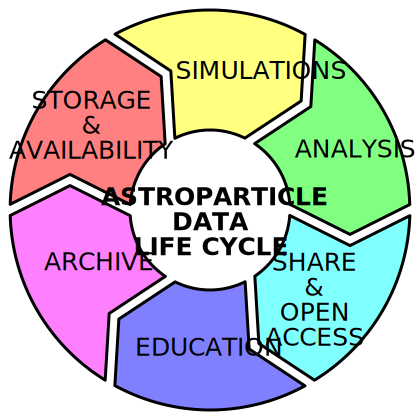
\includegraphics[width=1\textwidth]{pics/ADLC.pdf}
    \end{minipage}
\end{frame}

\begin{frame}{KASCADE Cosmic-ray Data Center (KCDC)}
 \textcolor{red}{TODO: provide the overview!}
\end{frame}

\begin{frame}{APPDS Architecture}
\begin{minipage}[c]{0.63\textwidth}
  \includegraphics[width=1\textwidth]{pics/arch_appds.png}
\end{minipage}
\hfill
\begin{minipage}[c]{0.36\textwidth}
  \small
  \begin{itemize}
    \setlength{\itemsep}{0pt}
%     \setlength{\parskip}{0pt}
    \item\textbf{Si} — local data storages;
    \item\textbf{Ini} — data sources of different types;
    \item\textbf{MDD} — metadata description;
    \item\textbf{Ei} — metadata extractors;
    \item\textbf{Ai} — adapters, provide API for data access;
    \item\textbf{TPL} — template library;
    \item\textbf{MD DB} — metadata database.
  \end{itemize}
\end{minipage}
\end{frame}



